\chapter{Scalable Graph Similarity}

In this chapter we provide a summary of our work on scalable graph similarity calculation.
This work stems from the general problem of determining the similarity between \emph{objects}
in a data set, which can take many forms: cosine similarity between
items embedded in a low-dimensional representation \cite{word2vec}, ...
\todo{A second thing here}, or as done
in this work, by modeling the problem as graph similarity calculation.
The use of the generic object term here is intentional, as our method is domain-agnostic
and can be applied in a variety of domains where a meaningful measure of correlation
between objects can be derived. In the paper we present examples from the linguistic,
music, and molecular biology domains.
In our approach we model the objects as nodes in graph and their interactions as edges,
weighted by a measure of correlation between the objects. In language for example, the
nodes would be words and the edges could be weighted by their mutual information \cite{mutual-information-nlp}.
We then compute the similarities between nodes by applying a transformation on this \emph{correlation graph}, to produce a graph which surfaces deeper,
semantic interactions which we term the \emph{similarity graph}.
In order to determine the similarity between objects in graph, we examine
their agreement in correlations to other objects: if two nodes are highly
correlated to similar sets of nodes, they are more likely to be similar themselves.

However, the computation of all-to-all similarities in a graph can quickly become
intractable for large graphs. The popular SimRank \cite{simrank} algorithm developed by 
Jen and Widom for this purpose
has a cubic time complexity with respect to the number of nodes in the graph.
Clearly then for large-scale graphs some form of approximation needs to be used
to make the computation feasible.

As in other works in this thesis, we apply a combination of using approximations to limit
the computational cost of the method, and develop a distributed algorithm that allows
us to scale-out learning and take advantage of modern computing clusters.

The first approximation we employ makes use a characteristic that many real-world datasets exhibit,
that is, there exists a long-tail distribution of interactions between items in a graph. These type
of ``small-world'' graphs, appear in areas like gene co-expression \cite{gene-small-world}, semantic networks \cite{semantic-small-world},
word co-occurrences \cite{words-small-world} and social networks (see \cite{barabasi-small-world} for further
examples).
This allows us to prune the input correlation graph significantly before transforming it,
while maintaining a controllable and small approximation error.

The second approximation has to do with the locality of the computation. Instead of trying
to solve the computationally intractable all-to-all similarity problem, we instead only look at
nodes that are one hop apart, keeping the computation local and dramatically limiting the number of
cost per node in the graph.
This approximation is what makes the distributed implementation of the algorithm efficient.
In order to compute for each pair of nodes in a neighborhood their common sets of correlated nodes,
we need only examine the common sets of incoming edges per node. By distributing our graph
using the id of the incoming nodes as a key we can perform this computation using a
self-join operation, which involves no communication of data in the cluster. As a result
we are able to scale the computation to massive datasets, as we show with our use of the
Google Books n-gram dataset, which corresponds to approximate 4\% of all the books ever
printed \cite{ngrams} (24.5 billion rows).



\section{Background} \todo{Compare to similarity learning methods}

In this section we will provide the necessary background knowledge that places our
work in the context of the wider research on similarity calculation.

\subsection{Using context as a measure of similarity}

\section{Main Findings}

\subsection{Method}

\subsubsection*{Definitions}


\subsubsection*{Similarity formula with example}

\subsubsection*{Concept Discover through community detection}

\subsubsection{Results}

In this section we provide a summary of the results presented in the paper,
and present previously unpublished results that bridge deep learning
with our methods to allow for end-to-end concept discovery from raw images.

\subsubsection*{Visual concepts through the combination of Deep Learning and graphs}

In this experiment we make use of a combination of deep neural networks and our
algorithm to uncover visual concepts from raw images. Deep neural networks
can be trained on massive datasets of images to recognize multiple objects
in an image \cite{deep-learning}. The networks' accuracy creates a unique opportunity
to generate visual concepts out of raw images: A network trained on labeled dataset
like ImageNet \cite{imagenet} can be used to generate labels from unlabeled raw images thus generating
a ``silver-standard'' dataset which we can use as input for our algorithm.

In our experiments we have used the OpenImages dataset \cite{openimages} which uses
multiple image classifiers to annotate images with labels from 19,794 different
classes. The complete training
dataset contains 9,011,219 images scraped from the Flickr service\footnote{\url{www.flickr.com}}, of complex scenes annotated with 8.4 objects per image on average.

We use the OpenImages data to create a correlation graph of objects: We form
a clique for every object that exists together in one image, creating a graph that represents
how objects commonly appear together in real images. Take for example the annotated
image shown in Figure \ref{fig:horse-hat}. The image is annotated with both the
\emph{horse} and \emph{cowboy hat} labels. All the labels in the image will form
a clique in our graph. Looking at another image, \ref{fig:hat-guitar} we can now
extend this graph, by connecting the \emph{cowboy hat} label with the \emph{guitar}
label, creating a second degree link between the \emph{horse} and \emph{guitar} labels.
By incorporating all such images, our correlation graph will have a representation of objects
that tend to appear together in the real world. Using this graph as input, we can apply our similarity
transformation to group together objects that belong to semantically similar classes
based on the similarity between the contexts in which they appear in, in the real world. 
Finally we can apply our community detection algorithm to group together items to form
visual concepts in the similarity graph.

To illustrate the uncovered concepts, we take the 30,000 most similar
pair-wise object similarities and present the output similarity graph in Figure \ref{fig:openimages-concepts}, where the colors indicate the uncovered concepts.
To ease presentation we provide two zoomed-in parts in Figure \ref{fig:openimage-zoom},
where we can see objects that can roughly be described as ``uniformed people'' are grouped
together in Figure \ref{fig:openimages-military}, and objects that relate to cameras
grouped together in Figure \ref{fig:openimages-cameras}.

Using our algorithm in combination with deep learning models, we can use the wealth of unlabeled
images that exist in services like Flickr to create visual concepts.

\begin{figure}
	\centering
	\begin{subfigure}{\textwidth}
		\centering
		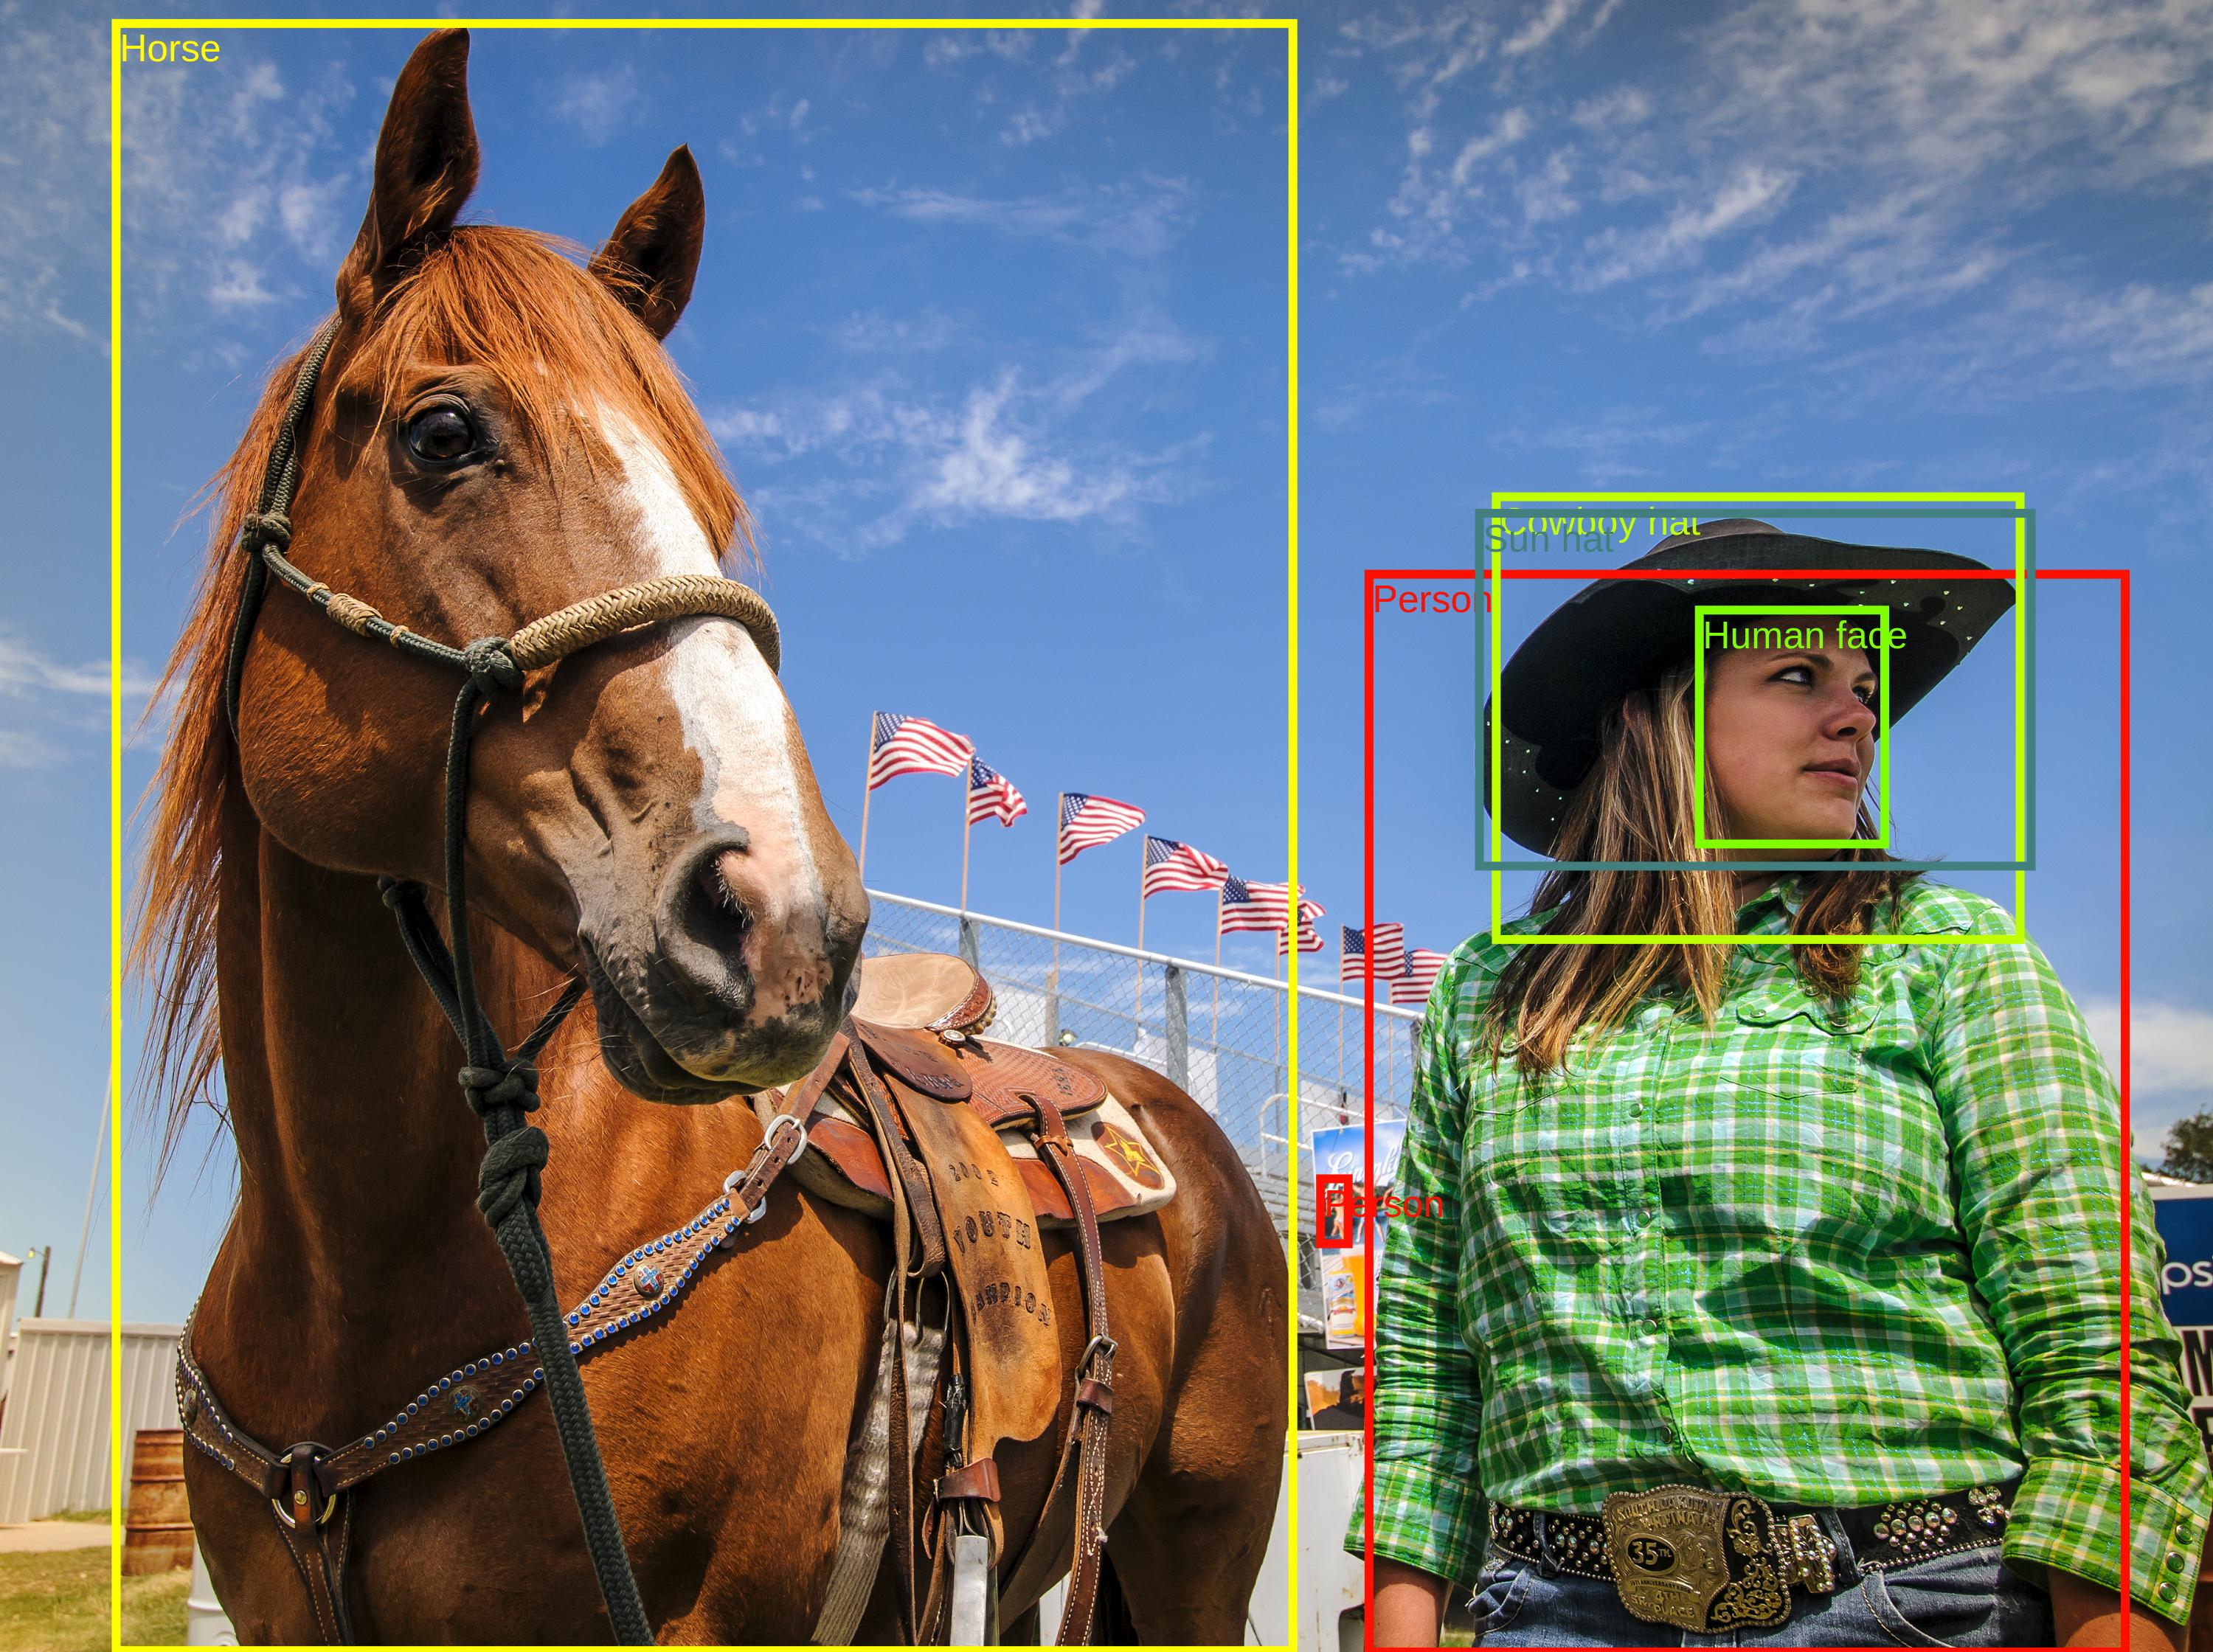
\includegraphics[width=0.9\textwidth]{horse-hat}
		\caption{An image that contains a horse and a cowboy hat.}
		\label{fig:horse-hat}
	\end{subfigure}
	~ %add desired spacing between images, e. g. ~, \quad, \qquad, \hfill etc.
	%(or a blank line to force the subfigure onto a new line)
	\begin{subfigure}{\textwidth}
		\centering
		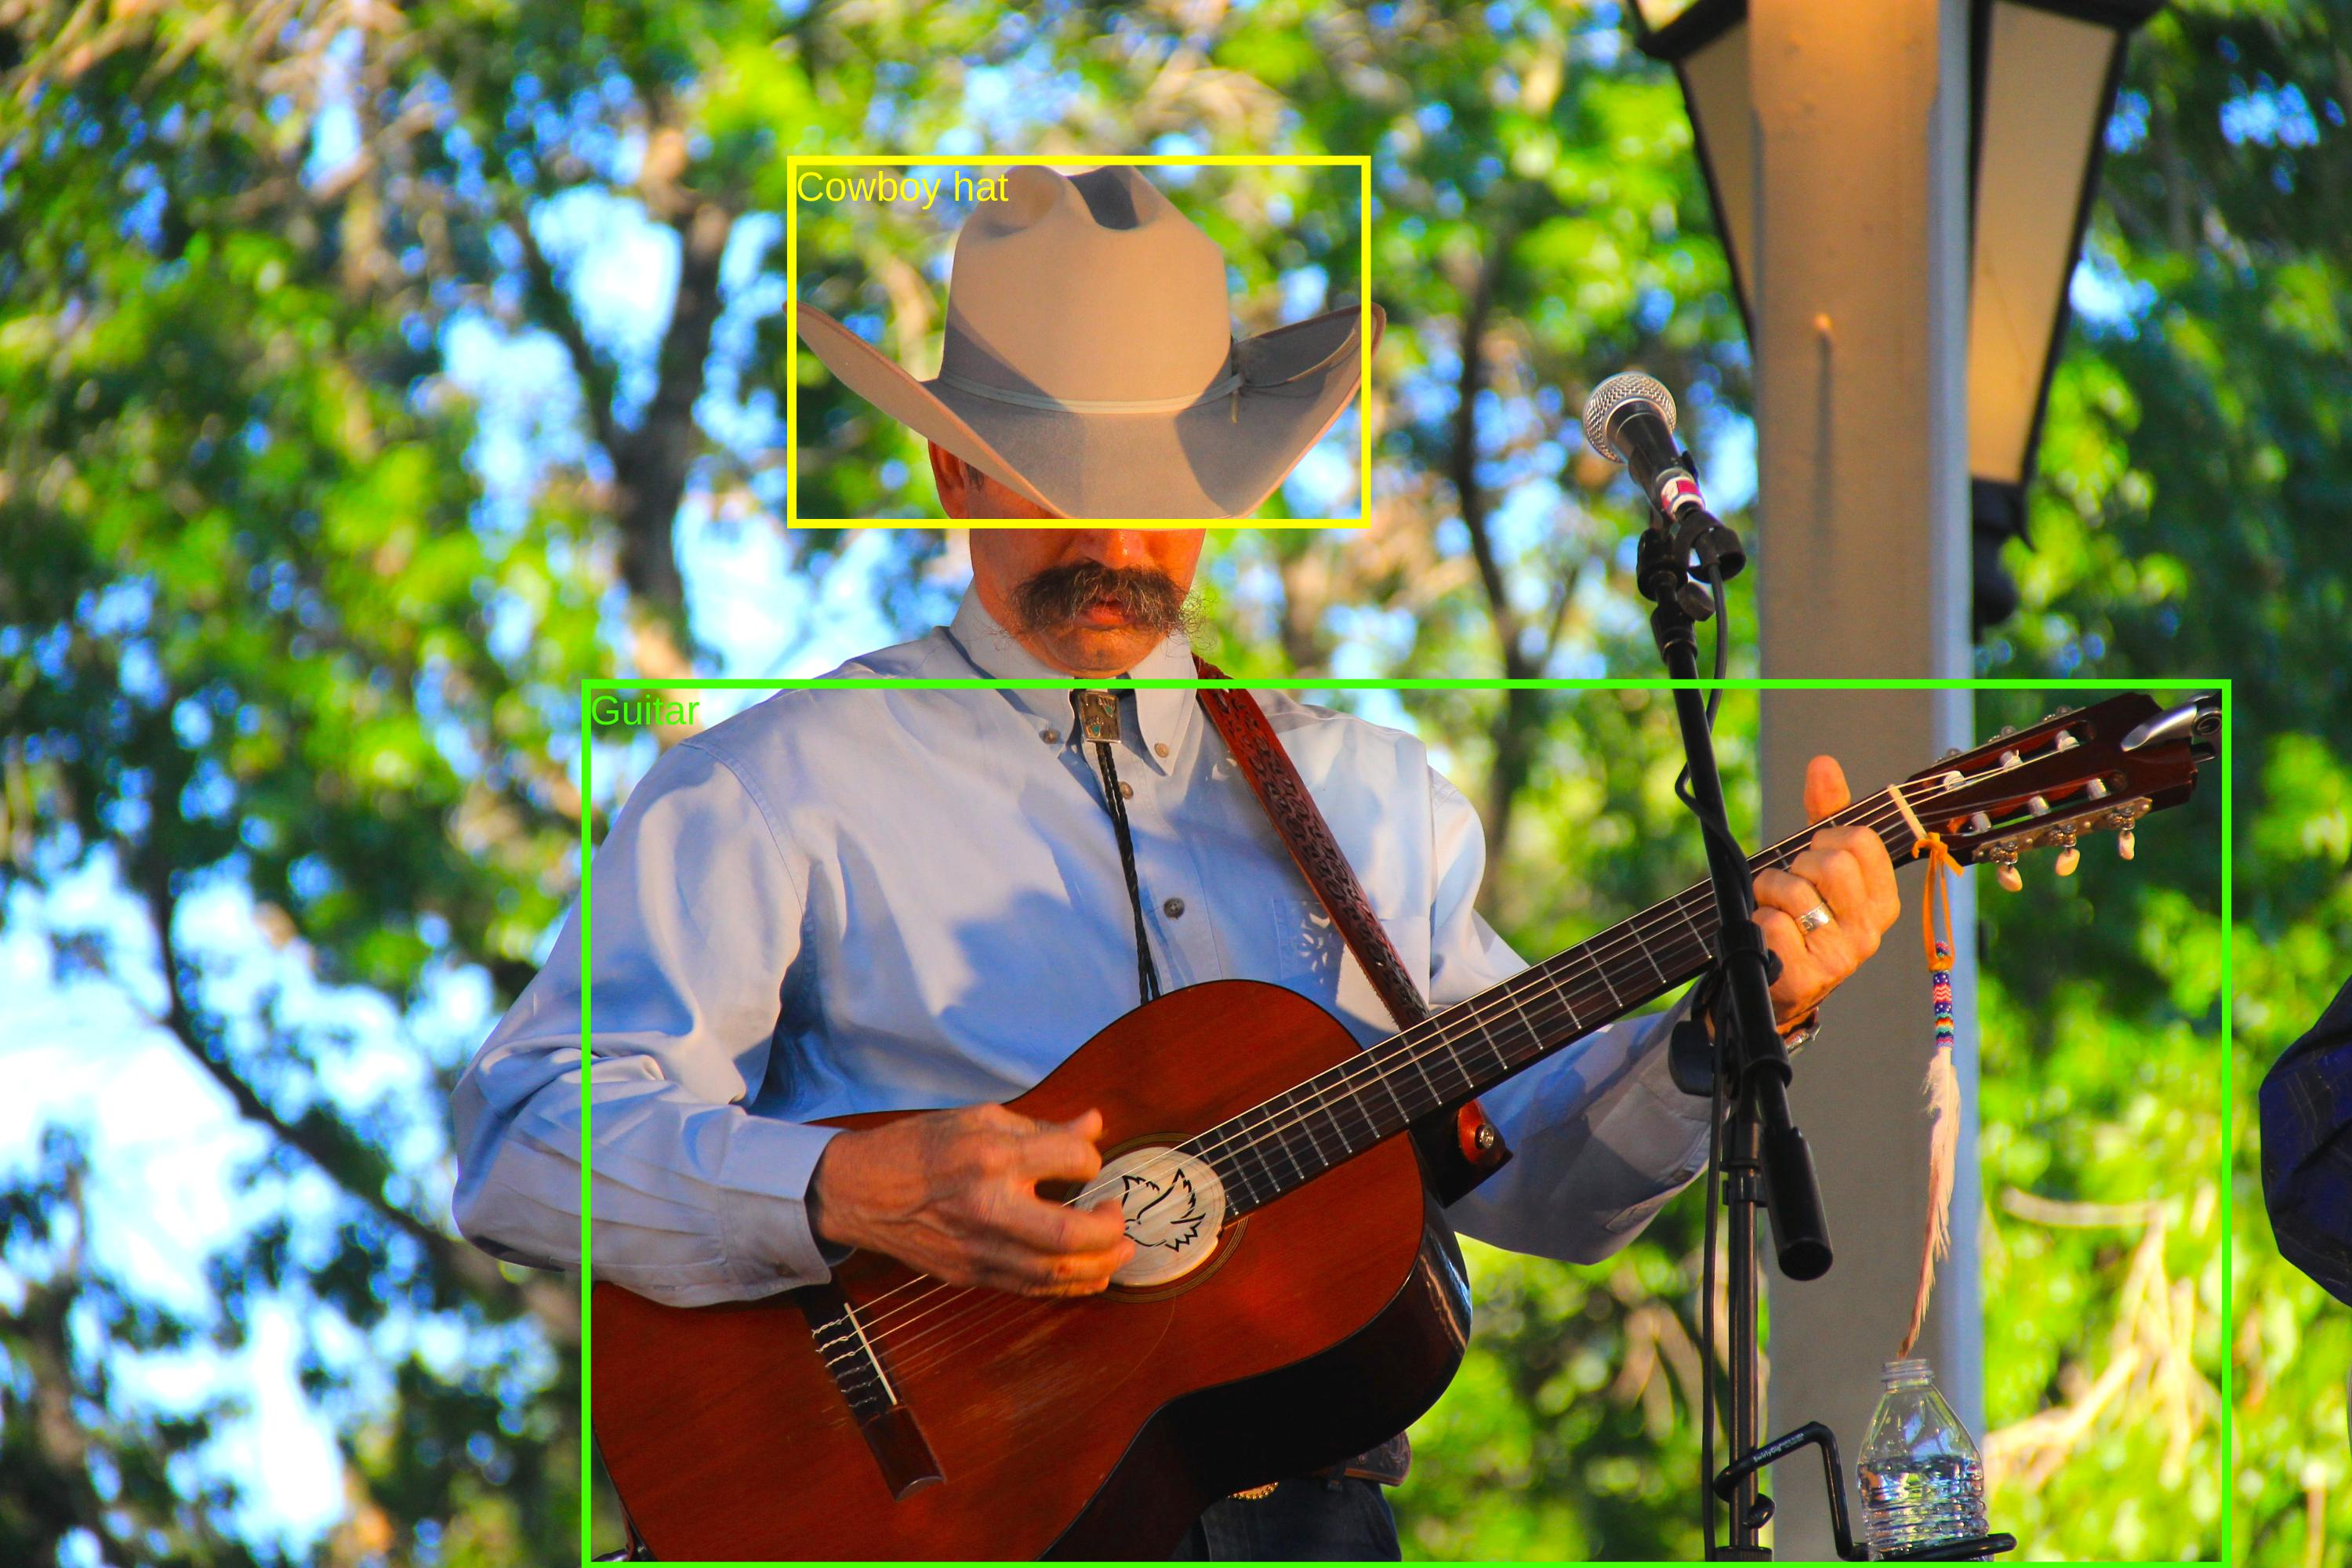
\includegraphics[width=0.9\textwidth]{hat-guitar}
		\caption{An image that contains a cowboy hat and a guitar.}
		\label{fig:hat-guitar}
	\end{subfigure}
	\caption{Examples of annotated images from the OpenImages dataset.}
	\label{fig:openimage-examples}
\end{figure}

\begin{figure}
	\centering
	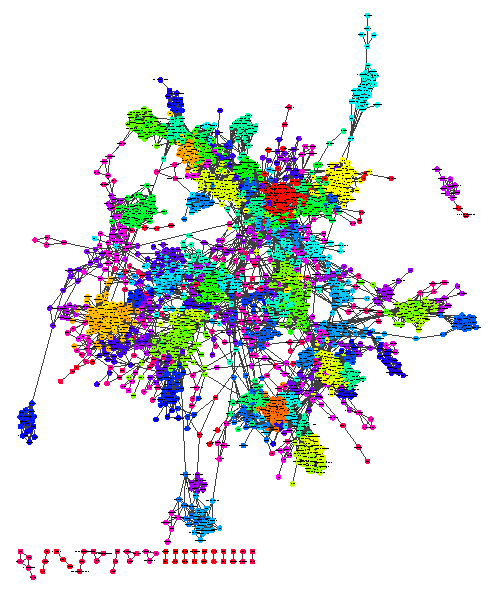
\includegraphics[width=\textwidth]{openimage-communities}
	\caption{The concepts uncovered by using the OpenImages data as input to our algorithm.
	The labels are legible through zooming in the electronic version. See Figure \ref{fig:openimage-zoom} for zoomed-in crops of the graph.}
	\label{fig:openimages-concepts}
\end{figure}


\begin{figure}
	\centering
	\begin{subfigure}{\textwidth}
		\centering
		
\includegraphics[height=0.44\textheight]{openimage-communities-military}
		\caption{A concept that brings together uniformed people and military objects.}
		\label{fig:openimages-military}
	\end{subfigure}
	 %add desired spacing between images, e. g. ~, \quad, \qquad, \hfill etc.
	%(or a blank line to force the subfigure onto a new line)
	\begin{subfigure}{\textwidth}
		\centering
		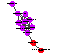
\includegraphics[height=0.44\textheight]{openimage-communities-cameras}
		\caption{A concept that groups together camera equipment.}
		\label{fig:openimages-cameras}
	\end{subfigure}
	\caption{Two visual concepts from the top-right corner of
		Figure \ref{fig:openimages-concepts}.}
	\label{fig:openimage-zoom}
\end{figure}
